 \let\negmedspace\undefined
\let\negthickspace\undefined
\documentclass[journal]{IEEEtran}
\usepackage[a5paper, margin=10mm, onecolumn]{geometry}
%\usepackage{lmodern} % Ensure lmodern is loaded for pdflatex
\usepackage{tfrupee} % Include tfrupee package

\setlength{\headheight}{1cm} % Set the height of the header box
\setlength{\headsep}{0mm}     % Set the distance between the header box and the top of the text

\usepackage{gvv-book}
\usepackage{gvv}
\usepackage{cite}
\usepackage{amsmath,amssymb,amsfonts,amsthm}
\usepackage{algorithmic}
\usepackage{graphicx}
\usepackage{textcomp}
\usepackage{xcolor}
\usepackage{txfonts}
\usepackage{listings}
\usepackage{enumitem}
\usepackage{mathtools}
\usepackage{gensymb}
\usepackage{comment}
\usepackage[breaklinks=true]{hyperref}
\usepackage{tkz-euclide} 
\usepackage{listings}
% \usepackage{gvv}                                        
\def\inputGnumericTable{}                                 
\usepackage[latin1]{inputenc}                                
\usepackage{color}                                            
\usepackage{array}                                            
\usepackage{longtable}                                       
\usepackage{calc}                                             
\usepackage{multirow}                                         
\usepackage{hhline}                                           
\usepackage{ifthen}                                           
\usepackage{lscape}
\usepackage{circuitikz}


\renewcommand{\thefigure}{\theenumi}
\renewcommand{\thetable}{\theenumi}
\setlength{\intextsep}{10pt} % Space between text and floats


\numberwithin{equation}{enumi}
\numberwithin{figure}{enumi}
\renewcommand{\thetable}{\theenumi}


% Marks the beginning of the document
\begin{document}
\bibliographystyle{IEEEtran}
\vspace{3cm}

\title{GATE 2014}
\author{EE25BTECH11060 - Namaswi Vajjala}
\maketitle

% (add your content here)
\begin{enumerate}
\item 
Choose the most appropriate phrase from the options given below to complete the following sentence. The aircraft take off as soon as its flight plan was filed.
\hfill{(GATE ME 2014)}
\begin{multicols}{2}
\begin{enumerate}
    \item  is allowed to
    \item will be allowed to
    \item was allowed to
    \item has been allowed to
\end{enumerate} 
\end{multicols}

\item  Read the statements:
All women are entrepreneurs.
Some women are doctors.
Which of the following conclusions can be logically inferred from the above statements?
\hfill{(GATE ME 2014)}
\begin{multicols}{2}
 \begin{enumerate}
        \item  All women are doctors
        \item All doctors are enterprenures
        \item All entrepreneurs are women
        \item some entrepreneurs are doctors
 \end{enumerate}
\end{multicols}

\item Choose the most appropriate word from the options given below to complete the following sentence.
Many ancient cultures attributed disease to supernatural causes. However, modern science has largely helped
\hfill{(GATE ME 2014)}
\begin{multicols}{4}
    \begin{enumerate}
        \item impel
        \item dispel
        \item propel
        \item repel
    \end{enumerate}
\end{multicols}

\item 
The statistics of runs scored in a series by four batsmen are provided in the following table. Who is the most consistent batsman of these four?
\hfill{(GATE ME 2014)}
 \begin{table}[h!]
\centering
\begin{tabular}{|c|c|c|}
\hline
\textbf{Batsman} & \textbf{Average} & \textbf{Standard deviation} \\
\hline
K & 31.2 & 5.21 \\
\hline
L & 46.0 & 6.35 \\
\hline
M & 54.4 & 6.22 \\
\hline
N & 17.9 & 5.90 \\
\hline
\end{tabular}
\end{table}

\begin{multicols}{4}
    \begin{enumerate}
        \item K
        \item L
        \item M
        \item N
    \end{enumerate}
\end{multicols}

\item what is the next number of series 12 35 81 173 357

\item Find the odd one from the following group:
W,E,K,O  \quad   I,Q,W,A \quad      F,N,T,X   \quad      N,V,B,D\\
 \begin{multicols}{4}
\begin{enumerate}
    \item W,E,K,O
    \item I,Q,W,A
    \item F,N,T,X
    \item N,V,B,D
\end{enumerate}   
\end{multicols}

\item For submitting tax returns, all resident males with annual income below Rs 10 lakh should fill up Form P and all resident females with income below Rs 8 lakh should fill up Form Q. All people with incomes above Rs 10 lakh should fill up Form R, except non residents with income above Rs 15 lakhs, who should fill up Form S. All others should fill Form T. An example of a person who should fill Form T is
\hfill{(GATE ME 2014)}
 \begin{enumerate}
\item a resident male with annual income Rs 9 lakh
\item a resident female with annual income Rs 9 lakh
\item  a non-resident male with annual income Rs 16 lakh
\item a non-resident female with annual income Rs 16 lakh
\end{enumerate}

\item A train that is 280 metres long, travelling at a uniform speed, crosses a platform in 60 seconds and passes a man standing on the platform in 20 seconds. What is the length of the platform in metres?\\
\hfill{(GATE ME 2014)}

\item 
The exports and imports (in crores of Rs.) of a country from 2000 to 2007 are given in the following bar chart. If the trade deficit is defined as excess of imports over exports, in which year is the trade deficit 1/5th of the exports?
\begin{figure}
    \centering
    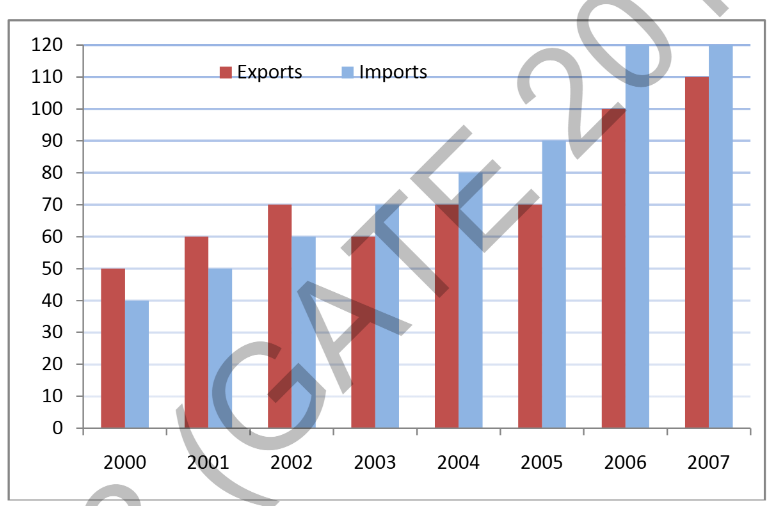
\includegraphics[width=0.7\columnwidth]{figs/fig2.1.png}
    \caption{Caption}
    \label{fig:2.1}
\end{figure}
\hfill{(GATE ME 2014)}
\begin{multicols}{4}
    \begin{enumerate}
        \item 2005
        \item 2004
        \item 2007
        \item 2006
    \end{enumerate}
\end{multicols}
\item You are given three coins: one has heads on both faces, the second has tails on both faces, and the third has a head on one face and a tail on the other. You choose a coin at random and toss it, and it comes up heads. The probability that the other face is tails is
\hfill{(GATE ME 2014)}
\begin{multicols}{4}
    \begin{enumerate}
        \item 1/4
        \item 1/3
        \item 1/2
        \item 2/3
    \end{enumerate}
\end{multicols}
\end{enumerate}

\newpage
\textbf{Q.1-Q.25 carry one mark each}
\begin{enumerate}

\item  Given that the determinant of matrix \( A = \begin{bmatrix} 1 & 3 & 0 \\ 2 & 6 & 4 \\ -1 & 0 &  2 \end{bmatrix} \) is -12,the determinant of the matrix \( A = \begin{bmatrix} 2 & 6 & 0 \\ 4 & 12 & 8 \\ -2 & 0 & 4 \end{bmatrix} \) is 
\hfill{(GATE ME 2014)}
 \begin{multicols}{4}
 \begin{enumerate}
         \item -96
         \item -24
         \item 24
         \item 96
     \end{enumerate}
 \end{multicols}
 \item 
 $\lim_{x \to 0} \frac{x - \sin x}{1 - \cos x}$ is
 \hfill{(GATE ME 2014)}
 \begin{multicols}{4}
\begin{enumerate}
 \item 0
 \item 1
 \item 3
 \item not defined
\end{enumerate}
 \end{multicols}
\item The argument of complex numbers $\frac{1+i}{1-i}$,where i is $\sqrt{-1}$, is
\hfill{(GATE ME 2014)}
\begin{multicols}{4}
    \begin{enumerate}
        \item $-\pi$
        \item $-\pi/2$
        \item $\pi/2$
        \item $\pi$
        \end{enumerate}
        \end{multicols}
\item The matrix form of linear system $\frac{dy}{dx}$=3x-5y and $\frac{dy
   }{dt}$=4x+8y is
\hfill{(GATE ME 2014)}
    \begin{multicols}{4}
    \begin{enumerate}
    \item 
    \begin{align*}
\frac{d}{dt}
\begin{Bmatrix}
x \\
y
\end{Bmatrix}
&=
\begin{bmatrix}
3 & -5 \\
4 & 8
\end{bmatrix}
\begin{Bmatrix}
x \\
y
\end{Bmatrix}
\end{align*}
\item \begin{align*}
\frac{d}{dt}
\begin{Bmatrix}
x \\
y
\end{Bmatrix}
&=
\begin{bmatrix}
3 & 8 \\
4 & -5
\end{bmatrix}
\begin{Bmatrix}
x \\
y
\end{Bmatrix}
\end{align*}
    \item \begin{align*}
\frac{d}{dt}
\begin{Bmatrix}
x \\
y
\end{Bmatrix}
&=
\begin{bmatrix}
4 & -5 \\
3 & 8
\end{bmatrix}
\begin{Bmatrix}
x \\
y
\end{Bmatrix}
\end{align*}

\item \begin{align*}
\frac{d}{dt}
\begin{Bmatrix}
x \\
y
\end{Bmatrix}
&=
\begin{bmatrix}
4 & 8 \\
3 & -5
\end{bmatrix}
\begin{Bmatrix}
x \\
y
\end{Bmatrix}
\end{align*}
\end{enumerate}
\end{multicols}

\item 
Which one of the following describes the relationship among the three vectors, 
\[
\hat{i} + \hat{j} + \hat{k}, \quad
\begin{aligned}
\vec{v}_1 &= 2\hat{i} + 3\hat{j} + \hat{k}, \\
\vec{v}_2 &= 5\hat{i} + 6\hat{j} + 4\hat{k}
\end{aligned}
\]

\hfill{(GATE ME 2014)}

\begin{enumerate}
    \item The vectors are mutually perpendicular
    \item The vectors are linearly dependent
    \item The vectors are linearly independent
    \item The vectors are unit vectors
\end{enumerate}
\item A circular rod of length 'L' and area of cross-section 'A' has a modulus of elasticity 'E' and
coefficient of thermal expansion 'a'. One end of the rod is fixed and other end is free. If the
temperature of the rod is increased by AT, then

\hfill{(GATE ME 2014)}

\begin{enumerate}
    
\item  stress developed in the rod is E a AT and strain developed in the rod is a AT
\item  both stress and strain developed in the rod are zero
\item  stress developed in the rod is zero and strain developed in the rod is a AT
\item  stress developed in the rod is E a AT and strain developed in the rod is zero

\end{enumerate}

\item A metallic rod of 500 mm length and 50 mm diameter, when subjected to a tensile force of 100 kN
at the ends, experiences an increase in its length by 0.5 mm and a reduction in its diameter by
0.015 mm. The Poisson's ratio of the rod material is

\hfill{(GATE ME 2014)}

\item 
Critical damping is the

\hfill{(GATE ME 2014)}

\begin{enumerate}
    \item largest amount of damping for which no oscillation occurs in free vibration
    \item largest amount of damping for which the motion is simple harmonic in free vibration
    \item  smallest amount of damping for which the motion is simple harmonic in free vibration
    \item smallest amount of damping for which the motion is simple harmonic for free vibration
    \end{enumerate}

\item A circular object of radius r rolls without slipping on a horizontal level floor with the center having
velocity V. The velocity at the point of contact between the object and the floor is
 
\hfill{(GATE ME 2014)}
\
    \begin{enumerate}
        \item zero
        \item V in the direction of motion
        \item  V opposite to the direction of motion
        \item V vertically upward from the floor
    \end{enumerate}

\item 
For the given statements:
I. Mating spur gear teeth is an example of higher pair
II. A revolute joint is an example of lower pair
Indicate the correct answer.

\hfill{(GATE ME 2014)}

\begin{enumerate}
    \item Both I and II are false
    \item I is true and II is false
\item  I is false and II is true
\item Both I and II are true
\end{enumerate}

\item A rigid link PQ is 2 m long and oriented at 20° to the horizontal as shown in the figure. The
magnitude and direction of velocity Vo, and the direction of velocity Vp are given. The magnitude
of Vp (in m/s) at this instant is
\begin{figure}[H]
    \centering
    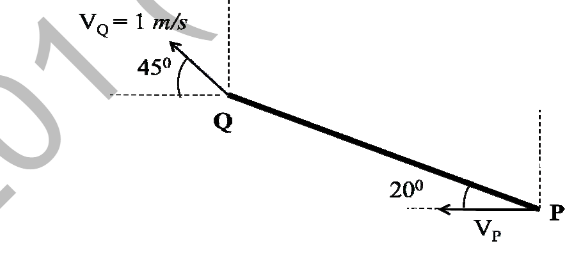
\includegraphics[width = 0.6\columnwidth]{figs/fig2.2.png}
    \caption*{}
    \label{fig:Q14}
\end{figure}

 \hfill{(GATE ME 2014)}
 
\begin{multicols}{4}
    \begin{enumerate}
        \item 2.14
        \item 1.89
        \item 1.21
        \item 0.96
    \end{enumerate}
\end{multicols}
\item Biot number signifies the ratio of

 \hfill{(GATE ME 2014)}
 
\begin{enumerate}
    \item convective resistance in the fluid to conductive resistance in the solid
\item  conductive resistance in the solid to convective resistance in the fluid
\item  inertia force to viscous force in the fluid
\item  buoyancy force to viscous force in the fluid
\end{enumerate}
\item The maximum theoretical work obtainable, when a system interacts to equilibrium with a reference
environment, is called

 \hfill{(GATE ME 2014)}
 
\begin{multicols}{4}
\begin{enumerate}
    \item entropy
    \item enthalpy
    \item energy
    \item rothalpy
    \end{enumerate}
    \end{multicols}
    \item Consider a two-dimensional laminar flow over a long cylinder as shown in the figure below.
\begin{figure}[H]
    \centering
    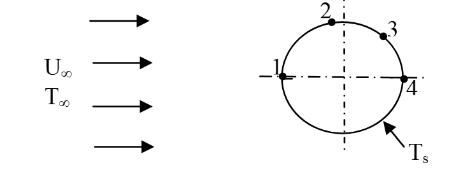
\includegraphics[width = 0.6\columnwidth]{figs/fig2.3.png}
    \caption*{}
    \label{fig:Q14}
\end{figure}

    
    The free stream velocity is U., and the free stream temperature T is lower than the cylinder
surface temperature Ts. The local heat transfer coefficient is minimum at point

 \hfill{(GATE ME 2014)}
 
\begin{multicols}{4}
    \begin{enumerate}
        \item 1
        \item 2
        \item 3
        \item 4
    \end{enumerate}
\end{multicols}
\item For a completely submerged body with centre of gravity 'G' and centre of buoyancy 'B', the
condition of stability will be

 \hfill{(GATE ME 2014)}
 
\begin{enumerate}
    \item G is located below B
    \item G is located above B
    \item G and B are coincident
    \item independent of locations of G and B
\end{enumerate}

\item In a power plant, water  $\brak{density=1000 kg/m^3}$ is pumped from 80 kPa to 3 MPa. The pump has an
isentropic efficiency of 0.85. Assuming that the temperature of the water remains the same, the
specific work  $\brak{in KJ}$ supplied to the pump is

 \hfill{(GATE ME 2014)}
 
\begin{enumerate}
    \item 0.34
    \item 2.48
    \item 2.92
    \item 3.43
\end{enumerate}
\item Which one of the following is CFG refrigreant

  \hfill{(GATE ME 2014)}
  
\begin{multicols}{4}
    \begin{enumerate}
        \item R744
        \item R290
        \item R502
        \item R718
    \end{enumerate}
\end{multicols}
\item The jobs arrive at a facility, for service, in a random manner. The probability distribution of number of arrivals of job of fixed time interval is 
 \hfill{(GATE ME 2014)}
 
\begin{multicols}{4}
    \begin{enumerate}
        \item Normal
        \item poisson
        \item erlang
        \item beta
    \end{enumerate}
\end{multicols}

\item 
In exponential smoothening method, which one of the following is true?

 \hfill{(GATE ME 2014)}
 
\begin{enumerate}
    \item $0 < a \le 1$ and high value of a is used for stable demand
\item$0 \le a \le 1$ and high value of a is used for unstable demand
\item  $a \ge 1$ and high value of a is used for stable demand
\item  $a \le 0$ and high value of a is used for unstable demand
\end{enumerate}
\item For machining a rectangular island represented by coordinates P $\brak{0,0}$ Q $\brak{100,0}$, R $\brak{100,50}$ and S $\brak{0,50}$ on a casting using CNC milling machine, an end mill with a diameter of 16 mm is used.The trajectory of the cutter centre to machine the island PQRS is

 \hfill{(GATE ME 2014)}
 
\begin{enumerate}   
    \item  $\brak{-8,-8},\ \brak{108,-8},\ \brak{108,58},\ \brak{-8,58},\ \brak{-8,-8}$
    \item  $\brak{8,8},\ \brak{94,8},\ \brak{94,44},\ \brak{8,44},\ \brak{8,8}$
    \item  $\brak{-8,8},\ \brak{94,0},\ \brak{94,44},\ \brak{8,44},\ \brak{-8,8}$
    \item  $\brak{0,0},\ \brak{100,0},\ \brak{100,50},\ \brak{50,0},\ \brak{0,0}$
\end{enumerate}

\item Which one of the following instruments is widely used to check and calibrate geometric features of
machine tools during their assembly?

 \hfill{(GATE ME 2014)}
 
\begin{enumerate}
    \item Ultrasonic probe
    \item Coordinate machine learning
    \item Laser interferometer
    \item Vernier callipers
\end{enumerate}
\item The major difficulty during welding of aluminium is due to its

 \hfill{(GATE ME 2014)}
 
\begin{enumerate}
    \item high tendency of oxidation
    \item higher thermal conductivity
\item low melting point
\item lower density
\end{enumerate}

\item The main cutting force acting on a tool during the turning (orthogonal cutting) operation of a metal
is 400 N. The turning was performed using 2 mm depth of cut and 0.1 mm/rev feed rate. The
specific cutting pressure $(in N/mm^2)$ is

 \hfill{(GATE ME 2014)}
 
\begin{multicols}{4}
\begin{enumerate}
    \item 1000
    \item 2000
    \item 3000
    \item 4000
\end{enumerate}
\end{multicols}

\item The process of reheating the martensitic steel to reduce its brittleness without any significant loss in
its hardness is

 \hfill{(GATE ME 2014)}
 
\begin{multicols}{4}
    \begin{enumerate}
        \item normalising
        \item annealing
\item quenching
\item  tempering
 \end{enumerate}
\end{multicols}
\item In solid-state welding, the contamination layers between the surfaces to be welded are removed by

 \hfill{(GATE ME 2014)}
 
\begin{multicols}{4}
\begin{enumerate}
    \item alcohol
    \item plastic deformation
    \item water jet
    \item sand blasting
\end{enumerate} 
\end{multicols}
 \textbf{Q.26-Q.55 carry two marks each }

  \item The integral 
    \[
    \oint_C \brak{y\,dx - x\,dy}
    \]
    is evaluated along the circle 
    \[
    x^2 + y^2 = \frac{1}{4}
    \]
    traversed in counter-clockwise direction. The integral is equal to:
    
 \hfill{(GATE ME 2014)}
 
    \begin{multicols}{2}
    \begin{enumerate}
        \item $0$
        \item $-\dfrac{\pi}{4}$
        \item $-\dfrac{\pi}{2}$
        \item $\dfrac{\pi}{4}$
     \end{enumerate}
    \end{multicols}

    \item If $y = f(x)$ is the solution of 
\begin{align*}
    \frac{d^2 y}{dx^2} = 0
\end{align*}
    with the boundary conditions 
    \[
    y = 5 \text{ at } x = 0, \quad \text{and} \quad \frac{dy}{dx} = 2 \text{ at } x = 10,
    \]
    then 
    \[
    f(15) = \underline{\hspace{2cm}}
    \]

    \item In the following table, $x$ is a discrete random variable and $p(x)$ is the probability density. The standard deviation of $x$ is:

    \[
    \begin{array}{|c|c|c|c|}
    \hline
    x & 1 & 2 & 3 \\
    \hline
    p(x) & 0.3 & 0.6 & 0.1 \\
    \hline
    \end{array}
    \]
    
 \hfill{(GATE ME 2014)}
 
    \begin{multicols}{2}
    \begin{enumerate}
    
        \item $0.18$
        \item $0.36$
        \item $0.54$
        \item $0.6$
    \end{enumerate}
    \end{multicols}

    \item Using the trapezoidal rule, and dividing the interval of integration into three equal subintervals, the definite integral
\begin{align*} 
    \int_{-1}^{1} |x|\, dx = \underline{\hspace{2cm}}   
\end{align*} 

\hfill{(GATE ME 2014)}

\item \begin{align*}
\text{The state of stress at a point is given by:} \\
\sigma_x &= -6~\text{MPa}, \\
\sigma_y &= 4~\text{MPa}, \\
\tau_{xy} &= -8~\text{MPa}.
\end{align*}

\noindent
\text{The tensile stress (in MPa) at the point is:}


 \hfill{(GATE ME 2014)}


\item A block R of mass 100 kg is placed on a block S of mass 150 kg as shown in the figure. Block R is tied to the wall by a massless and inextensible string PQ. If the coefficient of static friction for all surfaces is 0.4, the minimum force F $\brak{in KN}$ needed to move the block S is

\begin{figure}[H]
    \centering
    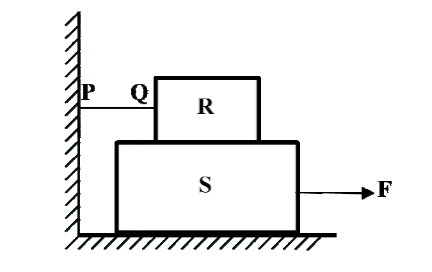
\includegraphics[width = 0.6\columnwidth]{figs/fig2.4.png}
    \caption*{}
    \label{fig:Q31}
\end{figure}

 \hfill{(GATE ME 2014)}
 
\begin{multicols}{4}
    \begin{enumerate}
        \item 0.69
        \item 0.88
        \item 0.98
        \item 1.37
    \end{enumerate}
\end{multicols}

\item A pair of spur gears with module 5 mm and a center distance of 450 mm is used for a speed
reduction of 5:1. The number of teeth on pinion is

 \hfill{(GATE ME 2014)}
 
\item Consider a cantilever beam, having negligible mass and uniform flexural rigidity, with length
0.01 m. The frequency of vibration of the beam, with a 0.5 kg mass attached at the free tip, is
100 Hz. The flexural rigidity $\brak{Nm^2}$ of the beam is

 \hfill{(GATE ME 2014)}
 
\item An ideal water jet with volume flow rate of 0.05 m3/s strikes a flat plate placed normal to its path
and exerts a force of 1000 N. Considering the density of water as 1000 kg/m3, the diameter $\brak{in mm}$
of the water jet is

 \hfill{(GATE ME 2014)}
 
\item A block weighing 200 N is in contact with a level plane whose coefficients of static and kinetic
friction are 0.4 and 0.2, respectively. The block is acted upon by a horizontal force $\brak{in newton}$
P=10t, where t denotes the time in seconds. The velocity $\brak{in m/s}$
 of the block attained after
10 seconds is

 \hfill{(GATE ME 2014)}
 
\item A slider crank mechanism has slider mass of 10 kg, stroke of 0.2 m and rotates with a uniform
angular velocity of 10 rad/s. The primary inertia forces of the slider are partially balanced by a
revolving mass of 6 kg at the crank, placed at a distance equal to crank radius. Neglect the mass of
connecting rod and crank. When the crank angle $\brak{with respect to slider axis}$ is 30°, the unbalanced
force $\brak{in newton}$ normal to the slider axis is

 \hfill{(GATE ME 2014)}

\item An offset slider-crank mechanism is shown in the figure at an instant. Conventionally, the Quick
Return Ratio $\brak{QRR}$ is considered to be greater than one. The value of QRR is


 \hfill{(GATE ME 2014)}
 
\begin{figure}[H]
    \centering
    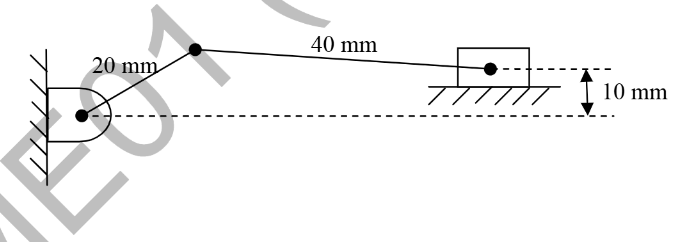
\includegraphics[width = 0.6\columnwidth]{figs/fig2.5.png}
    \caption*{}
    \label{fig:Q37}
\end{figure}

\item A rigid uniform rod AB of length L and mass m is hinged at C such that AC = L/3, CB = 2L/3. Ends
A and B are supported by springs of spring constant k. The natural frequency of the system is given
by
 \hfill{(GATE ME 2014)}
 
\begin{figure}[H]
    \centering
    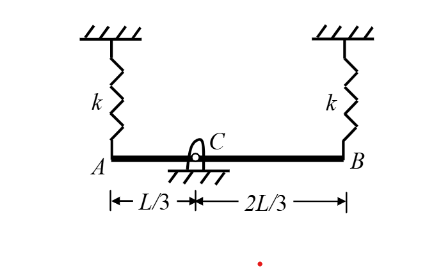
\includegraphics[width = 0.6\columnwidth]{figs/fig2.6.png}
    \caption*{}
    \label{fig:Q38}
\end{figure}
\begin{multicols}{4}
    \begin{enumerate}
        \item $\sqrt{k/2m}$
         \item $\sqrt{k/m}$
         \item $\sqrt{2k/m}$
         \item $\sqrt{5k/m}$
    \end{enumerate}
\end{multicols}

\item A hydrodynamic journal bearing is subject to 2000 N load at a rotational speed of 2000 rpm. Both
bearing bore diameter and length are 40 mm. If radial clearance is 20 um and bearing is lubricated
with an oil having viscosity 0.03 Pa.s, the Sommerfeld number of the bearing is

 \hfill{(GATE ME 2014)}
 
\item A 200 mm long, stress free rod at room temperature is held between two immovable rigid walls.
The temperature of the rod is uniformly raised by 250C. If the Young's modulus and coefficient of
thermal expansion are 200 GPa and 1x$10^{-5}$ \degree C, respectively, the magnitude of the longitudinal
stress $\brak{MPa}$ developed in the rod is

 \hfill{(GATE ME 2014)}
 
\item 1.5 kg of water is in saturated liquid state at 2 bar $\brak{vf = 0.001061 m3/kg, uf= 504.0 kJ/kg,hf= 505 kJ/kg}$. Heat is added in a constant pressure process till the temperature of water reaches 400\degree C .
$\brak{v=1.5493 m^3/kg, u=2967.0 kJ/kg, h= 3277.0 kJ/kg}$
The heat added $\brak{in KJ}$ in the process is

 \hfill{(GATE ME 2014)}

\item Consider one dimensional steady state heat conduction across a wall $\brak{as shown in figure below}$ of
thickness 30 mm and thermal conductivity 15 W/m.K. At x = 0, a constant heat flux,
q" = 1x$10^{5}$ $W/m^{2}$ is applied. On the other side of the wall, heat is removed from the wall by
convection with a fluid at  an$25\degree C$ and heat transfer coefficient of 250 $W/m^{2}$.K. The temperature
$\brak{in C}$, at x = 0 is
 \hfill{(GATE ME 2014)}

\item Water flows through a pipe having an inner radius of 10 mm at the rate of 36 kg/hr at $ 25 \degree C $. The viscosity of water at $25\degree C$ is 0.001 kg/m.s. The Reynolds number of the flow is

\hfill{(GATE ME 2014)}

\item For a fully developed flow of water in a pipe having diameter 10 cm, velocity 0.1 m/s and
kinematic viscosity  
 the value of Darcy friction factor is

\hfill{(GATE ME 2014)}

\item In a simple concentric shaft-bearing arrangement, the lubricant flows in the 2 mm gap between the
shaft and the bearing. The flow may be assumed to be a plane Couette flow with zero pressure
gradient. The diameter of the shaft is 100 mm and its tangential speed is 10 m/s. The dynamic
viscosity of the lubricant is 0.1 kg/m.s. The frictional resisting force $\brak{newton}$ per 100 mm length
of the bearing is
 \hfill{(GATE ME 2014)}

\item The non-dimensional fluid temperature profile near the surface of a convectively cooled flat plate is given by \begin{align}
\frac{T_W - T}{T_W - T_\infty} = a + b \frac{y}{L} + c \left( \frac{y}{L} \right)^2
\end{align}
where y is measured perpendicular to the plate, L is the plate

length, and a, b and c are arbitrary constants. Tw and T. are wall and ambient temperatures,
respectively. If the thermal conductivity of the fluid is k and the wall heat flux is q", the Nusselt number Nu =\begin{align}
\frac{q''}{T_W - T_\infty} \cdot \frac{L}{k}
\end{align}
is equal to
 \hfill{(GATE ME 2014)}
\begin{multicols}{4}
    \begin{enumerate}
        \item a
        \item b
        \item 2c
        \item $b+2c$
    \end{enumerate}
\end{multicols}


\item In an air-standard Otto cycle, air is supplied at 0.1 MPa and 308 K. The ratio of the specific heats
$\brak{y}$ and the specific gas constant $\brak{R}$ of air are 1.4 and 288.8 J/kg.K, respectively. If the compression
ratio is 8 and the maximum temperature in the cycle is 2660 K, the heat $\brak{in KJ/kg}$ supplied to the engine is

 \hfill{(GATE ME 2014)}
 
\item A reversible heat engine receives 2 kJ of heat from a reservoir at 1000 K and a certain amount of
heat from a reservoir at 800 K. It rejects 1 kJ of heat to a reservoir at 400 K. The net work output
$\brak{KJ}$ of the cycle is

 \hfill{(GATE ME 2014)}
 
\item An ideal reheat Rankine cycle operates between the pressure limits of 10 kPa and 8 MPa, with
reheat being done at 4 MPa. The temperature of steam at the inlets of both turbines is 500C and
the enthalpy of steam is 3185 kJ/kg at the exit of the high pressure turbine and 2247 kJ/kg at the
exit of low pressure turbine. The enthalpy of water at the exit from the pump is 191 kJ/kg. Use the
following table for relevant data. 
\begin{table}[h!]
\centering
\begin{tabular}{|c|c|c|c|c|}
\hline
\textbf{Superheated steam temperature} & \textbf{Pressure} & $\boldsymbol{v}$ & $\boldsymbol{h}$ & $\boldsymbol{s}$ \\
(°C) & (MPa) & (m$^3$/kg) & (kJ/kg) & (kJ/kg$\cdot$K) \\
\hline
500 & 4 & 0.08644 & 3446 & 7.0922 \\
500 & 8 & 0.04177 & 3399 & 6.7266 \\
\hline
\end{tabular}
\caption{Properties of superheated steam at 500°C for different pressures.}
\end{table}
disregarding the pump the current efficiency is 
 \hfill{(GATE ME 2014)}

\item Jobs arrive at a facility at an average rate of 5 in an 8 hour shift. The arrival of the jobs follows
Poisson distribution. The average service time of a job on the facility is 40 minutes. The service
time follows exponential distribution. Idle time (in hours) at the facility per shift will be
\hfill{(GATE ME 2014)}

\begin{multicols}{4}
    \begin{enumerate}
        \item $\frac{5}{7}$
         \item $\frac{14}{3}$
          \item $\frac{7}{5}$
           \item $\frac{10}{3}$
    \end{enumerate}
\end{multicols}

  
\item A metal rod of initial length Lo is subjected to a drawing process. The length of the rod at any
instant is given by the expression, $L(t)=L(1+t^2)$ , where t is the time in minutes. The true strain rate $\brak{in min^{-1}}$ at the end of one minute is

 \hfill{(GATE ME 2014)}
 
\item During pure orthogonal turning operation of a hollow cylindrical pipe, it is found that the thickness
of the chip produced is 0.5 mm. The feed given to the zero degree rake angle tool is 0.2 mm/rev.
The shear strain produced during the operation is

 \hfill{(GATE ME 2014)}

\item For the given assembly: 25 H7/g8, match Group A with Group B

\hfill{(GATE ME 2014)}

\begin{enumerate}
    \item P-I, Q-III, R-IV, S-II
    \item P-I, Q-IV, R-III, S-II
    \item P-II, Q-III, R-IV, S-I
\item  P-II, Q-IV, R-III, S-I
\end{enumerate}
 
\item 
If the Taylor's tool life exponent n is 0.2, and the tool changing time is 1.5 min, then the tool life$\brak{in min}$ for maximum production rate is 

 \hfill{(GATE ME 2014)}
 
\item An aluminium alloy $\brak{density 2600 kg/m^3}$ casting is to be produced. A cylindrical hole of 100 mm
diameter and 100 mm length is made in the casting using sand core $\brak{density 2600 kg/m^3}$. The net
buoyancy force $\brak{in newton}$ acting on the core is

 \hfill{(GATE ME 2014)}
\end{enumerate}
\end{document} 






